%% template.tex
%% from
%% bare_conf.tex
%% V1.4b
%% 2015/08/26
%% by Michael Shell
%% See:
%% http://www.michaelshell.org/
%% for current contact information.
%%
%% This is a skeleton file demonstrating the use of IEEEtran.cls
%% (requires IEEEtran.cls version 1.8b or later) with an IEEE
%% conference paper.
%%
%% Support sites:
%% http://www.michaelshell.org/tex/ieeetran/
%% http://www.ctan.org/pkg/ieeetran
%% and
%% http://www.ieee.org/

%%*************************************************************************
%% Legal Notice:
%% This code is offered as-is without any warranty either expressed or
%% implied; without even the implied warranty of MERCHANTABILITY or
%% FITNESS FOR A PARTICULAR PURPOSE!
%% User assumes all risk.
%% In no event shall the IEEE or any contributor to this code be liable for
%% any damages or losses, including, but not limited to, incidental,
%% consequential, or any other damages, resulting from the use or misuse
%% of any information contained here.
%%
%% All comments are the opinions of their respective authors and are not
%% necessarily endorsed by the IEEE.
%%
%% This work is distributed under the LaTeX Project Public License (LPPL)
%% ( http://www.latex-project.org/ ) version 1.3, and may be freely used,
%% distributed and modified. A copy of the LPPL, version 1.3, is included
%% in the base LaTeX documentation of all distributions of LaTeX released
%% 2003/12/01 or later.
%% Retain all contribution notices and credits.
%% ** Modified files should be clearly indicated as such, including  **
%% ** renaming them and changing author support contact information. **
%%*************************************************************************


% *** Authors should verify (and, if needed, correct) their LaTeX system  ***
% *** with the testflow diagnostic prior to trusting their LaTeX platform ***
% *** with production work. The IEEE's font choices and paper sizes can   ***
% *** trigger bugs that do not appear when using other class files.       ***                          ***
% The testflow support page is at:
% http://www.michaelshell.org/tex/testflow/

\documentclass[conference,final,]{IEEEtran}
% Some Computer Society conferences also require the compsoc mode option,
% but others use the standard conference format.
%
% If IEEEtran.cls has not been installed into the LaTeX system files,
% manually specify the path to it like:
% \documentclass[conference]{../sty/IEEEtran}





% Some very useful LaTeX packages include:
% (uncomment the ones you want to load)


% *** MISC UTILITY PACKAGES ***
%
%\usepackage{ifpdf}
% Heiko Oberdiek's ifpdf.sty is very useful if you need conditional
% compilation based on whether the output is pdf or dvi.
% usage:
% \ifpdf
%   % pdf code
% \else
%   % dvi code
% \fi
% The latest version of ifpdf.sty can be obtained from:
% http://www.ctan.org/pkg/ifpdf
% Also, note that IEEEtran.cls V1.7 and later provides a builtin
% \ifCLASSINFOpdf conditional that works the same way.
% When switching from latex to pdflatex and vice-versa, the compiler may
% have to be run twice to clear warning/error messages.






% *** CITATION PACKAGES ***
%
%\usepackage{cite}
% cite.sty was written by Donald Arseneau
% V1.6 and later of IEEEtran pre-defines the format of the cite.sty package
% \cite{} output to follow that of the IEEE. Loading the cite package will
% result in citation numbers being automatically sorted and properly
% "compressed/ranged". e.g., [1], [9], [2], [7], [5], [6] without using
% cite.sty will become [1], [2], [5]--[7], [9] using cite.sty. cite.sty's
% \cite will automatically add leading space, if needed. Use cite.sty's
% noadjust option (cite.sty V3.8 and later) if you want to turn this off
% such as if a citation ever needs to be enclosed in parenthesis.
% cite.sty is already installed on most LaTeX systems. Be sure and use
% version 5.0 (2009-03-20) and later if using hyperref.sty.
% The latest version can be obtained at:
% http://www.ctan.org/pkg/cite
% The documentation is contained in the cite.sty file itself.






% *** GRAPHICS RELATED PACKAGES ***
%
\ifCLASSINFOpdf
  % \usepackage[pdftex]{graphicx}
  % declare the path(s) where your graphic files are
  % \graphicspath{{../pdf/}{../jpeg/}}
  % and their extensions so you won't have to specify these with
  % every instance of \includegraphics
  % \DeclareGraphicsExtensions{.pdf,.jpeg,.png}
\else
  % or other class option (dvipsone, dvipdf, if not using dvips). graphicx
  % will default to the driver specified in the system graphics.cfg if no
  % driver is specified.
  % \usepackage[dvips]{graphicx}
  % declare the path(s) where your graphic files are
  % \graphicspath{{../eps/}}
  % and their extensions so you won't have to specify these with
  % every instance of \includegraphics
  % \DeclareGraphicsExtensions{.eps}
\fi
% graphicx was written by David Carlisle and Sebastian Rahtz. It is
% required if you want graphics, photos, etc. graphicx.sty is already
% installed on most LaTeX systems. The latest version and documentation
% can be obtained at:
% http://www.ctan.org/pkg/graphicx
% Another good source of documentation is "Using Imported Graphics in
% LaTeX2e" by Keith Reckdahl which can be found at:
% http://www.ctan.org/pkg/epslatex
%
% latex, and pdflatex in dvi mode, support graphics in encapsulated
% postscript (.eps) format. pdflatex in pdf mode supports graphics
% in .pdf, .jpeg, .png and .mps (metapost) formats. Users should ensure
% that all non-photo figures use a vector format (.eps, .pdf, .mps) and
% not a bitmapped formats (.jpeg, .png). The IEEE frowns on bitmapped formats
% which can result in "jaggedy"/blurry rendering of lines and letters as
% well as large increases in file sizes.
%
% You can find documentation about the pdfTeX application at:
% http://www.tug.org/applications/pdftex





% *** MATH PACKAGES ***
%
%\usepackage{amsmath}
% A popular package from the American Mathematical Society that provides
% many useful and powerful commands for dealing with mathematics.
%
% Note that the amsmath package sets \interdisplaylinepenalty to 10000
% thus preventing page breaks from occurring within multiline equations. Use:
%\interdisplaylinepenalty=2500
% after loading amsmath to restore such page breaks as IEEEtran.cls normally
% does. amsmath.sty is already installed on most LaTeX systems. The latest
% version and documentation can be obtained at:
% http://www.ctan.org/pkg/amsmath





% *** SPECIALIZED LIST PACKAGES ***
%
%\usepackage{algorithmic}
% algorithmic.sty was written by Peter Williams and Rogerio Brito.
% This package provides an algorithmic environment fo describing algorithms.
% You can use the algorithmic environment in-text or within a figure
% environment to provide for a floating algorithm. Do NOT use the algorithm
% floating environment provided by algorithm.sty (by the same authors) or
% algorithm2e.sty (by Christophe Fiorio) as the IEEE does not use dedicated
% algorithm float types and packages that provide these will not provide
% correct IEEE style captions. The latest version and documentation of
% algorithmic.sty can be obtained at:
% http://www.ctan.org/pkg/algorithms
% Also of interest may be the (relatively newer and more customizable)
% algorithmicx.sty package by Szasz Janos:
% http://www.ctan.org/pkg/algorithmicx




% *** ALIGNMENT PACKAGES ***
%
%\usepackage{array}
% Frank Mittelbach's and David Carlisle's array.sty patches and improves
% the standard LaTeX2e array and tabular environments to provide better
% appearance and additional user controls. As the default LaTeX2e table
% generation code is lacking to the point of almost being broken with
% respect to the quality of the end results, all users are strongly
% advised to use an enhanced (at the very least that provided by array.sty)
% set of table tools. array.sty is already installed on most systems. The
% latest version and documentation can be obtained at:
% http://www.ctan.org/pkg/array


% IEEEtran contains the IEEEeqnarray family of commands that can be used to
% generate multiline equations as well as matrices, tables, etc., of high
% quality.




% *** SUBFIGURE PACKAGES ***
%\ifCLASSOPTIONcompsoc
%  \usepackage[caption=false,font=normalsize,labelfont=sf,textfont=sf]{subfig}
%\else
%  \usepackage[caption=false,font=footnotesize]{subfig}
%\fi
% subfig.sty, written by Steven Douglas Cochran, is the modern replacement
% for subfigure.sty, the latter of which is no longer maintained and is
% incompatible with some LaTeX packages including fixltx2e. However,
% subfig.sty requires and automatically loads Axel Sommerfeldt's caption.sty
% which will override IEEEtran.cls' handling of captions and this will result
% in non-IEEE style figure/table captions. To prevent this problem, be sure
% and invoke subfig.sty's "caption=false" package option (available since
% subfig.sty version 1.3, 2005/06/28) as this is will preserve IEEEtran.cls
% handling of captions.
% Note that the Computer Society format requires a larger sans serif font
% than the serif footnote size font used in traditional IEEE formatting
% and thus the need to invoke different subfig.sty package options depending
% on whether compsoc mode has been enabled.
%
% The latest version and documentation of subfig.sty can be obtained at:
% http://www.ctan.org/pkg/subfig




% *** FLOAT PACKAGES ***
%

%\usepackage{fixltx2e}
% fixltx2e, the successor to the earlier fix2col.sty, was written by
% Frank Mittelbach and David Carlisle. This package corrects a few problems
% in the LaTeX2e kernel, the most notable of which is that in current
% LaTeX2e releases, the ordering of single and double column floats is not
% guaranteed to be preserved. Thus, an unpatched LaTeX2e can allow a
% single column figure to be placed prior to an earlier double column
% figure.
% Be aware that LaTeX2e kernels dated 2015 and later have fixltx2e.sty's
% corrections already built into the system in which case a warning will
% be issued if an attempt is made to load fixltx2e.sty as it is no longer
% needed.
% The latest version and documentation can be found at:
% http://www.ctan.org/pkg/fixltx2e


%\usepackage{stfloats}
% stfloats.sty was written by Sigitas Tolusis. This package gives LaTeX2e
% the ability to do double column floats at the bottom of the page as well
% as the top. (e.g., "\begin{figure*}[!b]" is not normally possible in
% LaTeX2e). It also provides a command:
%\fnbelowfloat
% to enable the placement of footnotes below bottom floats (the standard
% LaTeX2e kernel puts them above bottom floats). This is an invasive package
% which rewrites many portions of the LaTeX2e float routines. It may not work
% with other packages that modify the LaTeX2e float routines. The latest
% version and documentation can be obtained at:
% http://www.ctan.org/pkg/stfloats
% Do not use the stfloats baselinefloat ability as the IEEE does not allow
% \baselineskip to stretch. Authors submitting work to the IEEE should note
% that the IEEE rarely uses double column equations and that authors should try
% to avoid such use. Do not be tempted to use the cuted.sty or midfloat.sty
% packages (also by Sigitas Tolusis) as the IEEE does not format its papers in
% such ways.
% Do not attempt to use stfloats with fixltx2e as they are incompatible.
% Instead, use Morten Hogholm'a dblfloatfix which combines the features
% of both fixltx2e and stfloats:
%
% \usepackage{dblfloatfix}
% The latest version can be found at:
% http://www.ctan.org/pkg/dblfloatfix




% *** PDF, URL AND HYPERLINK PACKAGES ***
%
%\usepackage{url}
% url.sty was written by Donald Arseneau. It provides better support for
% handling and breaking URLs. url.sty is already installed on most LaTeX
% systems. The latest version and documentation can be obtained at:
% http://www.ctan.org/pkg/url
% Basically, \url{my_url_here}.




% *** Do not adjust lengths that control margins, column widths, etc. ***
% *** Do not use packages that alter fonts (such as pslatex).         ***
% There should be no need to do such things with IEEEtran.cls V1.6 and later.
% (Unless specifically asked to do so by the journal or conference you plan
% to submit to, of course. )



%% BEGIN MY ADDITIONS %%


\usepackage{longtable,booktabs}
\usepackage{graphicx}
% We will generate all images so they have a width \maxwidth. This means
% that they will get their normal width if they fit onto the page, but
% are scaled down if they would overflow the margins.
\makeatletter
\def\maxwidth{\ifdim\Gin@nat@width>\linewidth\linewidth
\else\Gin@nat@width\fi}
\makeatother
\let\Oldincludegraphics\includegraphics
\renewcommand{\includegraphics}[1]{\Oldincludegraphics[width=\maxwidth]{#1}}

\usepackage[unicode=true]{hyperref}

\hypersetup{
            pdftitle={IEEE template for starwars analysis},
            pdfkeywords={keyword 1, keyword 2},
            pdfborder={0 0 0},
            breaklinks=true}
\urlstyle{same}  % don't use monospace font for urls

% Pandoc toggle for numbering sections (defaults to be off)
\setcounter{secnumdepth}{0}

% Pandoc syntax highlighting
\usepackage{color}
\usepackage{fancyvrb}
\newcommand{\VerbBar}{|}
\newcommand{\VERB}{\Verb[commandchars=\\\{\}]}
\DefineVerbatimEnvironment{Highlighting}{Verbatim}{commandchars=\\\{\}}
% Add ',fontsize=\small' for more characters per line
\usepackage{framed}
\definecolor{shadecolor}{RGB}{248,248,248}
\newenvironment{Shaded}{\begin{snugshade}}{\end{snugshade}}
\newcommand{\AlertTok}[1]{\textcolor[rgb]{0.94,0.16,0.16}{#1}}
\newcommand{\AnnotationTok}[1]{\textcolor[rgb]{0.56,0.35,0.01}{\textbf{\textit{#1}}}}
\newcommand{\AttributeTok}[1]{\textcolor[rgb]{0.77,0.63,0.00}{#1}}
\newcommand{\BaseNTok}[1]{\textcolor[rgb]{0.00,0.00,0.81}{#1}}
\newcommand{\BuiltInTok}[1]{#1}
\newcommand{\CharTok}[1]{\textcolor[rgb]{0.31,0.60,0.02}{#1}}
\newcommand{\CommentTok}[1]{\textcolor[rgb]{0.56,0.35,0.01}{\textit{#1}}}
\newcommand{\CommentVarTok}[1]{\textcolor[rgb]{0.56,0.35,0.01}{\textbf{\textit{#1}}}}
\newcommand{\ConstantTok}[1]{\textcolor[rgb]{0.00,0.00,0.00}{#1}}
\newcommand{\ControlFlowTok}[1]{\textcolor[rgb]{0.13,0.29,0.53}{\textbf{#1}}}
\newcommand{\DataTypeTok}[1]{\textcolor[rgb]{0.13,0.29,0.53}{#1}}
\newcommand{\DecValTok}[1]{\textcolor[rgb]{0.00,0.00,0.81}{#1}}
\newcommand{\DocumentationTok}[1]{\textcolor[rgb]{0.56,0.35,0.01}{\textbf{\textit{#1}}}}
\newcommand{\ErrorTok}[1]{\textcolor[rgb]{0.64,0.00,0.00}{\textbf{#1}}}
\newcommand{\ExtensionTok}[1]{#1}
\newcommand{\FloatTok}[1]{\textcolor[rgb]{0.00,0.00,0.81}{#1}}
\newcommand{\FunctionTok}[1]{\textcolor[rgb]{0.00,0.00,0.00}{#1}}
\newcommand{\ImportTok}[1]{#1}
\newcommand{\InformationTok}[1]{\textcolor[rgb]{0.56,0.35,0.01}{\textbf{\textit{#1}}}}
\newcommand{\KeywordTok}[1]{\textcolor[rgb]{0.13,0.29,0.53}{\textbf{#1}}}
\newcommand{\NormalTok}[1]{#1}
\newcommand{\OperatorTok}[1]{\textcolor[rgb]{0.81,0.36,0.00}{\textbf{#1}}}
\newcommand{\OtherTok}[1]{\textcolor[rgb]{0.56,0.35,0.01}{#1}}
\newcommand{\PreprocessorTok}[1]{\textcolor[rgb]{0.56,0.35,0.01}{\textit{#1}}}
\newcommand{\RegionMarkerTok}[1]{#1}
\newcommand{\SpecialCharTok}[1]{\textcolor[rgb]{0.00,0.00,0.00}{#1}}
\newcommand{\SpecialStringTok}[1]{\textcolor[rgb]{0.31,0.60,0.02}{#1}}
\newcommand{\StringTok}[1]{\textcolor[rgb]{0.31,0.60,0.02}{#1}}
\newcommand{\VariableTok}[1]{\textcolor[rgb]{0.00,0.00,0.00}{#1}}
\newcommand{\VerbatimStringTok}[1]{\textcolor[rgb]{0.31,0.60,0.02}{#1}}
\newcommand{\WarningTok}[1]{\textcolor[rgb]{0.56,0.35,0.01}{\textbf{\textit{#1}}}}


% Pandoc header

\providecommand{\tightlist}{%
  \setlength{\itemsep}{0pt}\setlength{\parskip}{0pt}}

%% END MY ADDITIONS %%


\hyphenation{op-tical net-works semi-conduc-tor}

\begin{document}
%
% paper title
% Titles are generally capitalized except for words such as a, an, and, as,
% at, but, by, for, in, nor, of, on, or, the, to and up, which are usually
% not capitalized unless they are the first or last word of the title.
% Linebreaks \\ can be used within to get better formatting as desired.
% Do not put math or special symbols in the title.
\title{IEEE template for starwars analysis}

% author names and affiliations
% use a multiple column layout for up to three different
% affiliations

\author{

%% ---- classic IEEETrans wide authors' list ----------------
 % -- end affiliation.wide
%% ----------------------------------------------------------



%% ---- classic IEEETrans one column per institution --------
 %% -- beg if/affiliation.institution-columnar
\IEEEauthorblockN{
  %% -- beg for/affiliation.institution.author
Advika Battini %% -- end for/affiliation.institution.author
}
\IEEEauthorblockA{School of Informatics and Data Science\\
University of Washington\\
Seattle, Washington
\\ece@uw.edu
}
\and
\IEEEauthorblockN{
  %% -- beg for/affiliation.institution.author
Homer Simpson %% -- end for/affiliation.institution.author
}
\IEEEauthorblockA{Twentieth Century Fox\\
Seattle, USA
  %% -- beg for/affiliation.institution.author
\\homer@thesimpsons.com
 %% -- end for/affiliation.institution.author
}
\and
\IEEEauthorblockN{
  %% -- beg for/affiliation.institution.author
Montgomery Scott %% -- end for/affiliation.institution.author
}
\IEEEauthorblockA{Starfleet Academy\\
San Francisco, California 96678-2391
  %% -- beg for/affiliation.institution.author
 %% -- end for/affiliation.institution.author
}
 %% -- end for/affiliation.institution
 %% -- end if/affiliation.institution-columnar
%% ----------------------------------------------------------





%% ---- one column per author, classic/default IEEETrans ----
 %% -- end if/affiliation.institution-columnar
%% ----------------------------------------------------------

}

% conference papers do not typically use \thanks and this command
% is locked out in conference mode. If really needed, such as for
% the acknowledgment of grants, issue a \IEEEoverridecommandlockouts
% after \documentclass

% for over three affiliations, or if they all won't fit within the width
% of the page, use this alternative format:
%
%\author{\IEEEauthorblockN{Michael Shell\IEEEauthorrefmark{1},
%Homer Simpson\IEEEauthorrefmark{2},
%James Kirk\IEEEauthorrefmark{3},
%Montgomery Scott\IEEEauthorrefmark{3} and
%Eldon Tyrell\IEEEauthorrefmark{4}}
%\IEEEauthorblockA{\IEEEauthorrefmark{1}School of Electrical and Computer Engineering\\
%Georgia Institute of Technology,
%Atlanta, Georgia 30332--0250\\ Email: see http://www.michaelshell.org/contact.html}
%\IEEEauthorblockA{\IEEEauthorrefmark{2}Twentieth Century Fox, Springfield, USA\\
%Email: homer@thesimpsons.com}
%\IEEEauthorblockA{\IEEEauthorrefmark{3}Starfleet Academy, San Francisco, California 96678-2391\\
%Telephone: (800) 555--1212, Fax: (888) 555--1212}
%\IEEEauthorblockA{\IEEEauthorrefmark{4}Tyrell Inc., 123 Replicant Street, Los Angeles, California 90210--4321}}




% use for special paper notices
%\IEEEspecialpapernotice{(Invited Paper)}




% make the title area
\maketitle

% As a general rule, do not put math, special symbols or citations
% in the abstract
\begin{abstract}
Week 4 in class activity
\end{abstract}

% keywords
\begin{IEEEkeywords}
keyword 1; keyword 2
\end{IEEEkeywords}

% use for special paper notices



% make the title area
\maketitle

% no keywords

% For peer review papers, you can put extra information on the cover
% page as needed:
% \ifCLASSOPTIONpeerreview
% \begin{center} \bfseries EDICS Category: 3-BBND \end{center}
% \fi
%
% For peerreview papers, this IEEEtran command inserts a page break and
% creates the second title. It will be ignored for other modes.
\IEEEpeerreviewmaketitle


\hypertarget{introduction}{%
\section{Introduction}\label{introduction}}

This demo file is intended to serve as a ``starter file'' for IEEE
conference papers produced under \LaTeX~using IEEEtran.cls version 1.8b
and later. I wish you the best of success.

\hypertarget{importing-libraries-first}{%
\subsection{Importing libraries
first\ldots{}}\label{importing-libraries-first}}

\begin{Shaded}
\begin{Highlighting}[]
\KeywordTok{library}\NormalTok{(tidyverse)}
\end{Highlighting}
\end{Shaded}

\hypertarget{in-this-activity-the-following-will-be-done}{%
\subsubsection{In this activity, the following will be
done:}\label{in-this-activity-the-following-will-be-done}}

\begin{enumerate}
\def\labelenumi{\arabic{enumi}.}
\tightlist
\item
  Uses starwars dataset \& tidyverse. \newline
\item
  Has a plot and table (no need for captions and cross-reference because
  this is hard with some templates) \newline
\item
  Has two in-text citations using bibtex \newline
\item
  Has a user-friendly, polished structure5.Has a set-up chunk, with 3+
  settings \newline
\item
  Uses code from an external R script file and knitr::read\_chunk()
  \newline
\item
  Uses a template from the rticles/papaja/tufte pkg or similar
  tufte::tufte\_html is a good option if you get LaTeX errors with other
  templates. You can delete the code and text in the template, but don't
  remove any YAML. \newline
\item
  Uses knitr caching on at least one chunk Setup chunk with 3+ settings
  and reading external code \newline
\end{enumerate}

\hypertarget{plotting}{%
\section{Plotting}\label{plotting}}

\hypertarget{using-external-r-code-and-plotting-a-figure}{%
\subsubsection{Using external R code and plotting a
figure}\label{using-external-r-code-and-plotting-a-figure}}

\begin{verbatim}
#> [1] "list is below:"
#> [1] -2 -1  0  1  2
\end{verbatim}

\begin{figure}
\centering
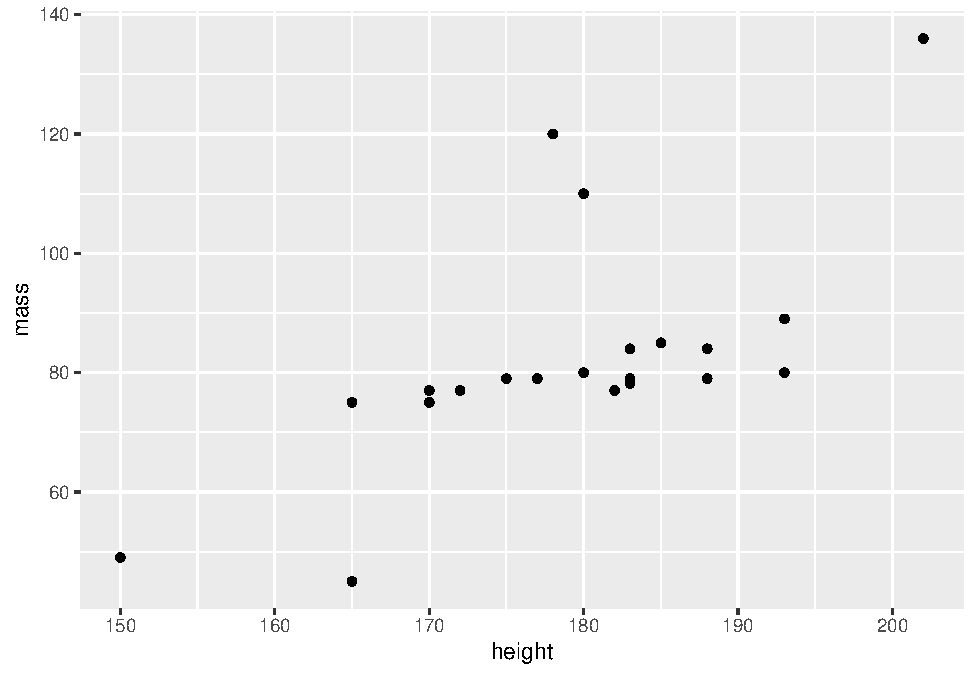
\includegraphics{my_template_files/figure-latex/starwarsplot-1.pdf}
\caption{A ggplot of starwars stuff}
\end{figure}

\hypertarget{using-caching}{%
\subsubsection{Using caching}\label{using-caching}}

\begin{verbatim}
#> [1] 1 2 3 4
\end{verbatim}

\hypertarget{benefits-of-parametrization}{%
\section{Benefits of
Parametrization}\label{benefits-of-parametrization}}

Parameterized reports extend the reproducibility of R Markdown by
allowing us to specify one or more parameters to customize the analysis.
This is useful if we want to create a report template that can be reused
across multiple similar scenarios. Examples may include: • Showing
results for a specific geographic location. \newline • Running a report
that covers a specific time period. \newline • Running a single analysis
multiple times for different assumptions. \newline • Controlling the
behavior of knitr (e.g., specify if you want the code to be displayed in
one version of the output and not displayed in another). \newline

\hypertarget{conclusion}{%
\section{Conclusion}\label{conclusion}}

This is the end of the week 4 in class activity.

\hypertarget{acknowledgment}{%
\section{Acknowledgment}\label{acknowledgment}}

The authors would like to thank Rstudio

The summary table is as follows: \onecolumn

\begin{longtable}[]{@{}lrr@{}}
\caption{A knitr kable table of starwars data}\tabularnewline
\toprule
name & height & mass\tabularnewline
\midrule
\endfirsthead
\toprule
name & height & mass\tabularnewline
\midrule
\endhead
Luke Skywalker & 172 & 77.0\tabularnewline
Darth Vader & 202 & 136.0\tabularnewline
Leia Organa & 150 & 49.0\tabularnewline
Owen Lars & 178 & 120.0\tabularnewline
Beru Whitesun lars & 165 & 75.0\tabularnewline
Biggs Darklighter & 183 & 84.0\tabularnewline
Obi-Wan Kenobi & 182 & 77.0\tabularnewline
Anakin Skywalker & 188 & 84.0\tabularnewline
Wilhuff Tarkin & 180 & NA\tabularnewline
Han Solo & 180 & 80.0\tabularnewline
Wedge Antilles & 170 & 77.0\tabularnewline
Jek Tono Porkins & 180 & 110.0\tabularnewline
Palpatine & 170 & 75.0\tabularnewline
Boba Fett & 183 & 78.2\tabularnewline
Lando Calrissian & 177 & 79.0\tabularnewline
Lobot & 175 & 79.0\tabularnewline
Mon Mothma & 150 & NA\tabularnewline
Arvel Crynyd & NA & NA\tabularnewline
Qui-Gon Jinn & 193 & 89.0\tabularnewline
Finis Valorum & 170 & NA\tabularnewline
Shmi Skywalker & 163 & NA\tabularnewline
Mace Windu & 188 & 84.0\tabularnewline
Gregar Typho & 185 & 85.0\tabularnewline
Cordé & 157 & NA\tabularnewline
Cliegg Lars & 183 & NA\tabularnewline
Dormé & 165 & NA\tabularnewline
Dooku & 193 & 80.0\tabularnewline
Bail Prestor Organa & 191 & NA\tabularnewline
Jango Fett & 183 & 79.0\tabularnewline
Jocasta Nu & 167 & NA\tabularnewline
Raymus Antilles & 188 & 79.0\tabularnewline
Finn & NA & NA\tabularnewline
Rey & NA & NA\tabularnewline
Poe Dameron & NA & NA\tabularnewline
Padmé Amidala & 165 & 45.0\tabularnewline
\bottomrule
\end{longtable}

\twocolumn

\hypertarget{bibliography-styles}{%
\section{Bibliography styles}\label{bibliography-styles}}

Here are some sample references: Gareau et al. (2011) , Clarkson et al.
(2017) , Feynman and Vernon Jr. (1963) , (Dirac 1953).

\newpage

\hypertarget{references}{%
\section*{References}\label{references}}
\addcontentsline{toc}{section}{References}

\hypertarget{refs}{}
\leavevmode\hypertarget{ref-clarkson2017human}{}%
Clarkson, Chris, Zenobia Jacobs, Ben Marwick, Richard Fullagar, Lynley
Wallis, Mike Smith, Richard G Roberts, et al. 2017. ``Human Occupation
of Northern Australia by 65,000 Years Ago.'' \emph{Nature} 547 (7663).
Nature Publishing Group: 306--10.

\leavevmode\hypertarget{ref-Dirac1953888}{}%
Dirac, P.A.M. 1953. ``The Lorentz Transformation and Absolute Time.''
\emph{Physica} 19 (1--12): 888--96.
\url{https://doi.org/10.1016/S0031-8914(53)80099-6}.

\leavevmode\hypertarget{ref-Feynman1963118}{}%
Feynman, R.P, and F.L Vernon Jr. 1963. ``The Theory of a General Quantum
System Interacting with a Linear Dissipative System.'' \emph{Annals of
Physics} 24: 118--73.
\url{https://doi.org/10.1016/0003-4916(63)90068-X}.

\leavevmode\hypertarget{ref-gareau2011bacterial}{}%
Gareau, Mélanie G, Eytan Wine, David M Rodrigues, Joon Ho Cho, Mark T
Whary, Dana J Philpott, Glenda MacQueen, and Philip M Sherman. 2011.
``Bacterial Infection Causes Stress-Induced Memory Dysfunction in
Mice.'' \emph{Gut} 60 (3). BMJ Publishing Group: 307--17.

\end{document}


